\documentclass[12pt,fleqn]{article}
\setlength{\parindent}{0pt}
\usepackage{graphicx}
\usepackage{cancel}
\usepackage{listings}
\usepackage[latin5]{inputenc}
\usepackage{color}
\setlength{\parskip}{8pt}
\setlength{\parsep}{0pt}
\setlength{\headsep}{0pt}
\setlength{\topskip}{0pt}
\setlength{\topmargin}{0pt}
\setlength{\topsep}{0pt}
\setlength{\partopsep}{0pt}
\setlength{\mathindent}{0cm}

\begin{document}
Cok Degiskenli Calculus - Ders 20

Cizgi entegrallerini is hesabinda gormustuk. $\vec{F}$ tarafindan $C$
egrisi uzerinde yapilan isi

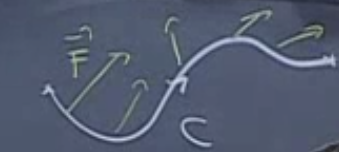
\includegraphics[height=2cm]{20_1.png}

\[ \int_C \vec{F} \cdot d\vec{r} =  \int_C \vec{F} \cdot \vec{T} ds \]

olarak gormustuk. Esitligin sagi birim teget vektoru kullanarak ayni hesabi
gosteriyor, $ds$ ise egri uzunlugu $s$'ten ortaya cikiyor. Diger bir form

\[ = \int_C M dx + N dy \]

ki $\vec{F} = <M,N>$ olmak uzere. 

Ornek 

Soyle bir vektor alani veriyorum

\[ \vec{F} = <y,x> \]

Bu alanin neye benzedigi cok bariz degil, ama bu alanin bir bilgisayar
cizimi altta

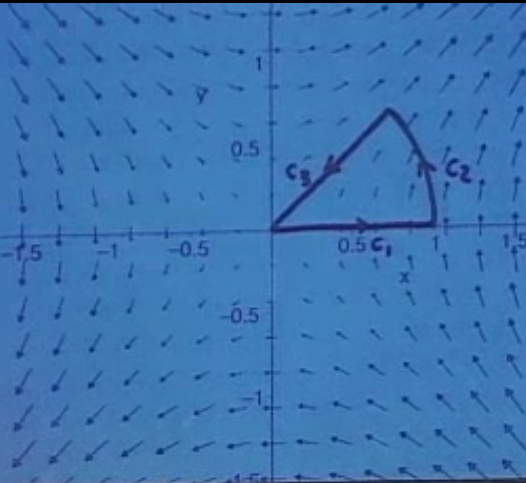
\includegraphics[height=5cm]{20_2.png}

Diyelim ki bu vektor alaninda orijinden baslayarak $c_1,c_2,c_3$
vektorlerini takip ederek hareket ettigimde yapilan isi hesaplamak
istiyorum. $c_1$ duz, $c_2$ birim cember uzerinde bir parca, $0 \le \theta
\le \pi / 4$ 
olmak uzere, ve $c_3$ tekrar duz. Yani 

\[ c = c_1 + c_2 + c_3 \]

O zaman is hesap entegralinin uc parcasi olacak. Her parca $i$ icin 

\[ \int_{C_i} y dx + x dy\]

gerekiyor. 

1) x ekseni, $(0,0)$'dan $(1,0)$'a. 

\[ y = 0, \ dy = 0 \]

\[ \int_{C_1} y dx + x dy = 0 \ dx + 0 = 0\]

Cizgi entegrali cok basit yani. Bu sifir sonucunu baska sekilde de
gorebilirdik, vektor alanina bakarsak x eksenine her zaman dik oldugunu
gorururz. O zaman $\vec{F}\cdot \vec{T}$ hep sifir sonucunu verecektir. 













\end{document}
